
\chapter{Leyes de Kirchhoff generalizadas}


En el caso de un doblete de fermiónes $\Xi$, el símbolo  $\dagger$ se usa para denotar el conjugado de fermiones de Weyl. El doblete adjunto en ese caso se puede definir como
\begin{align}
\label{eq:Xiadj}
 \widetilde{\Xi}=i\tau_2 \begin{pmatrix}
                  \Xi_1^{\dagger}\\
                  \Xi_2^{\dagger}\\
                \end{pmatrix}
=& \begin{pmatrix}
                  \Xi_2^{\dagger}\\
                 -\Xi_1^{\dagger}\\
                \end{pmatrix}
\end{align}
Para evitar confusiones con los invariantes $SU(2)$, usaremos entonces la definición de producto escalar en el espacio $SU(2)$ para escribir los correspondientes invariantes, por ejemplo
\begin{align}
  \widetilde{\Xi}\cdot \overline{\sigma}^{\mu}\Xi=\epsilon_{ab}\,\widetilde{\Xi}^{a}\overline{\sigma}^{\mu}\Xi^{b}\,.
\end{align}

Para evitar confusión con el conjugado de espinores de Weyl, usaremos el producto escalar con la métrica $SU(2)$ para escribir los correspondientes invariantes.


\section{Resumén de productos escalares}

\begin{frame}[fragile,allowframebreaks]

\begin{table}
  \centering
   \begin{tabular}{lll}
    Nombre & Símbolo & $\operatorname{SU(N)}$ \\\hline
    $N$-plete escalar & $\Psi$ & $U \Psi$ \\
    anti-$N$-plete escalar & $\Psi^\dagger $ & $\Psi^\dagger U^\dagger $ \\\hline
    \end{tabular}\hspace{3cm}
   \begin{tabular}{lll}
    Nombre & Símbolo & Lorentz \\\hline
    fotón & $A^\mu$ & ${\Lambda^\mu}_\nu A^\nu$ \\
    derivada & $\partial_\mu$ & $\partial_\nu {\left(\Lambda^{-1}\right)^\nu}_\mu$ \\\hline
  \end{tabular}
  \caption{
       Productos escalares: $\Psi^\dagger \Psi$,  \hspace{5cm}
      $\partial_\mu A^\nu \partial^\mu A_\nu=g^{\mu\alpha}g_{\nu \beta} \partial_\mu A^\nu \partial_{\alpha} A^{\beta} $
}
  \label{tab:fermionlr}
\end{table}
donde,
 $g_{\alpha\beta}={\Lambda^{\mu}}_{\alpha}\,g_{\mu\nu}{\Lambda^{\nu}}_{\beta}\,$,
  $g^{\mu\nu}={\left( \Lambda^{-1} \right)^{\mu}}_{\alpha}\,g^{\alpha\beta} {\left( \Lambda^{-1} \right)^{\nu}}_{\beta}\,$.


\begin{table}
  \centering
  \begin{tabular}{llll}
    Nombre & Símbolo & Lorentz & $U(1)$\\\hline\hline
    $e_L$: electrón izquierdo & $\xi_{\alpha}$ & ${\left[ S \right]_{\alpha}}^{\beta}\xi_{\beta}$ & $e^{i\theta}\xi$\\
   $\left( e_R \right)^{\dagger}=e^{\dagger}_L$: positrón izquierdo&$\eta^{\alpha}$& $\eta^\beta{\left[  S^{-1}  \right]_{\beta}}^{\alpha}$ & $\eta\, e^{-i\theta}$\\ \hline    
    $\left( e_L \right)^{\dagger}=e^{\dagger}_R$: positrón derecho   & $\left( \xi_{\alpha} \right)^{\dagger}=\xi^{\dagger}_{\dot{\alpha}}$ &
     $\xi^{\dagger}_{\dot{\beta}}{\left[{S^{\dagger}}\right]^{\dot{\beta}}}_{\dot{\alpha}}$ & $\xi^\dagger e^{-i\theta}$\\
   $e_R$: electrón derecho   & $\left( \eta^{\alpha} \right)^{\dagger}=\eta^{\dagger\;\dot{\alpha}}$ & ${\left[ \left( S^{-1} \right)^\dagger \right]^{\dot{\alpha}}}_{\dot{\beta}}\eta^{\dagger\;\dot{\beta}}$& $e^{i\theta}\eta^\dagger$\\\hline\hline
  \end{tabular}
  \caption{Escalar de Dirac: $\eta^{\alpha}\xi_{\alpha}+ \xi^{\dagger}_{\dot{\alpha}}\eta^{\dagger\;\dot{\alpha  }} $. Ya que: $ S^\dagger\overline{\sigma}^\mu S={\Lambda^\mu}_\nu\overline{\sigma}^\nu$:
  $i\xi_{\dot{\alpha}} \overline{\sigma}^{\dot{\alpha} \alpha} \partial_{\mu} \xi_{\alpha} $}
  \label{tab:fermionlr}
\end{table}

\end{frame}

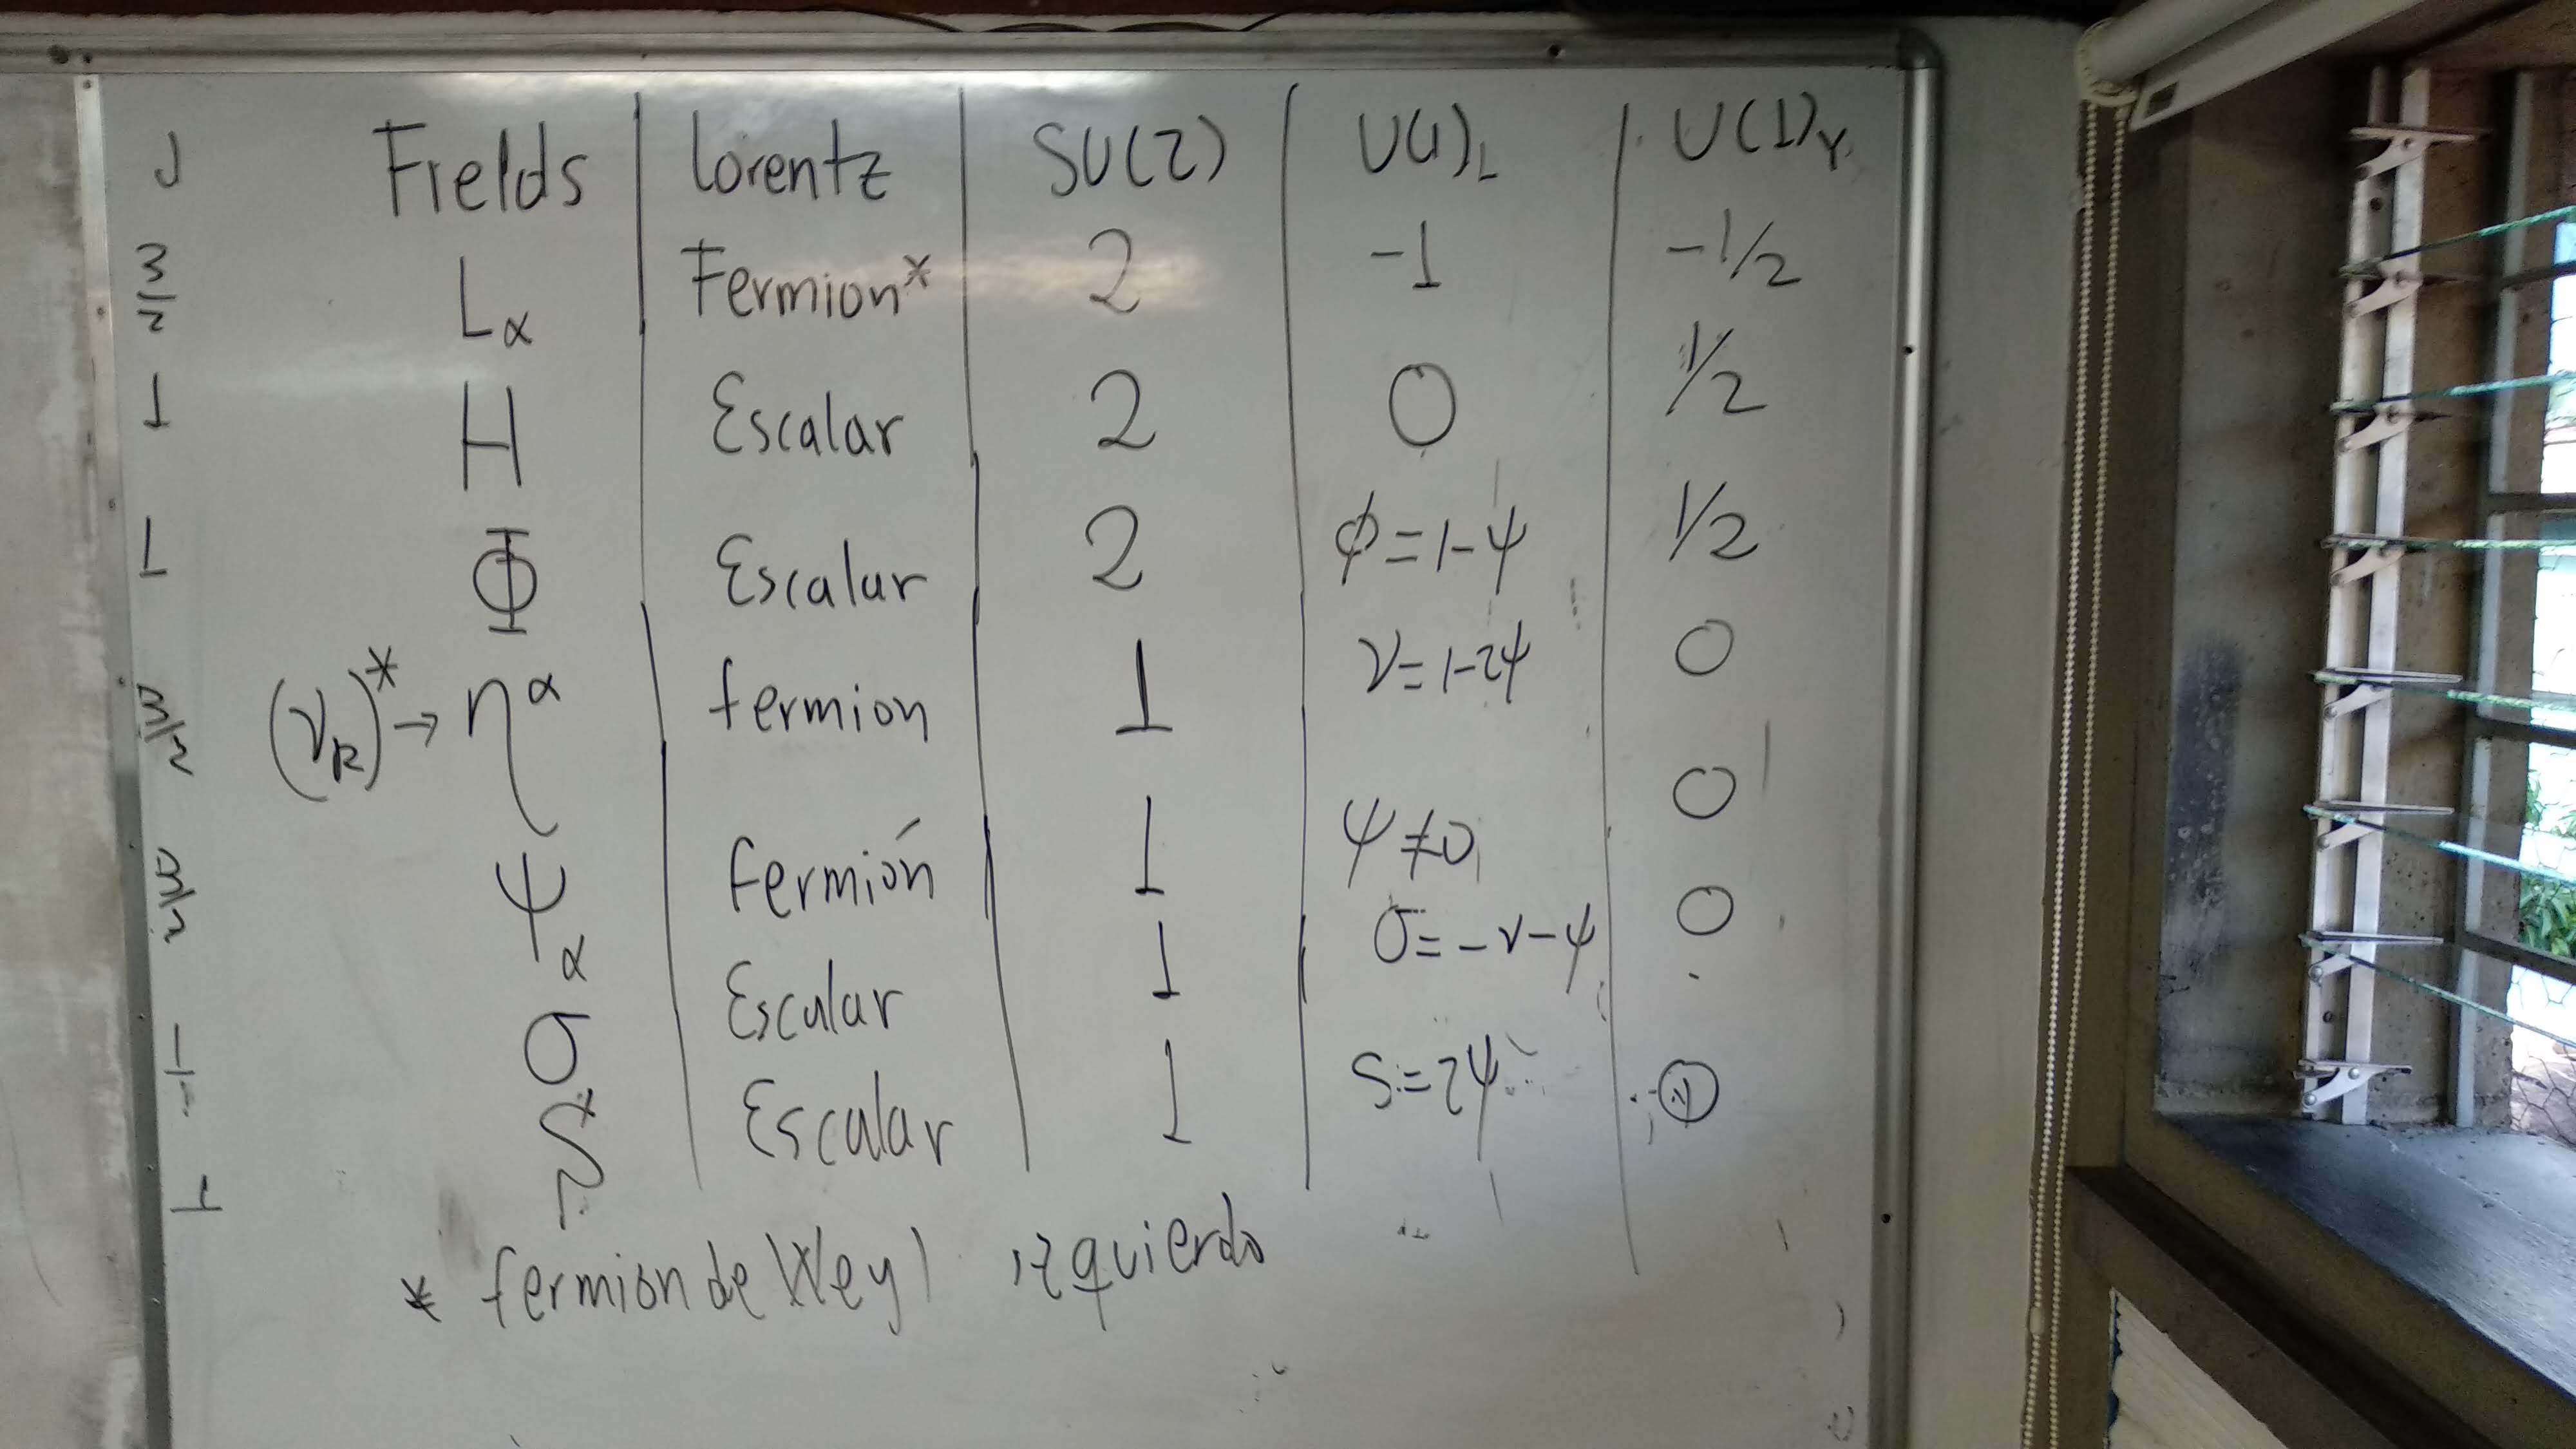
\includegraphics[scale=0.1]{tabla}

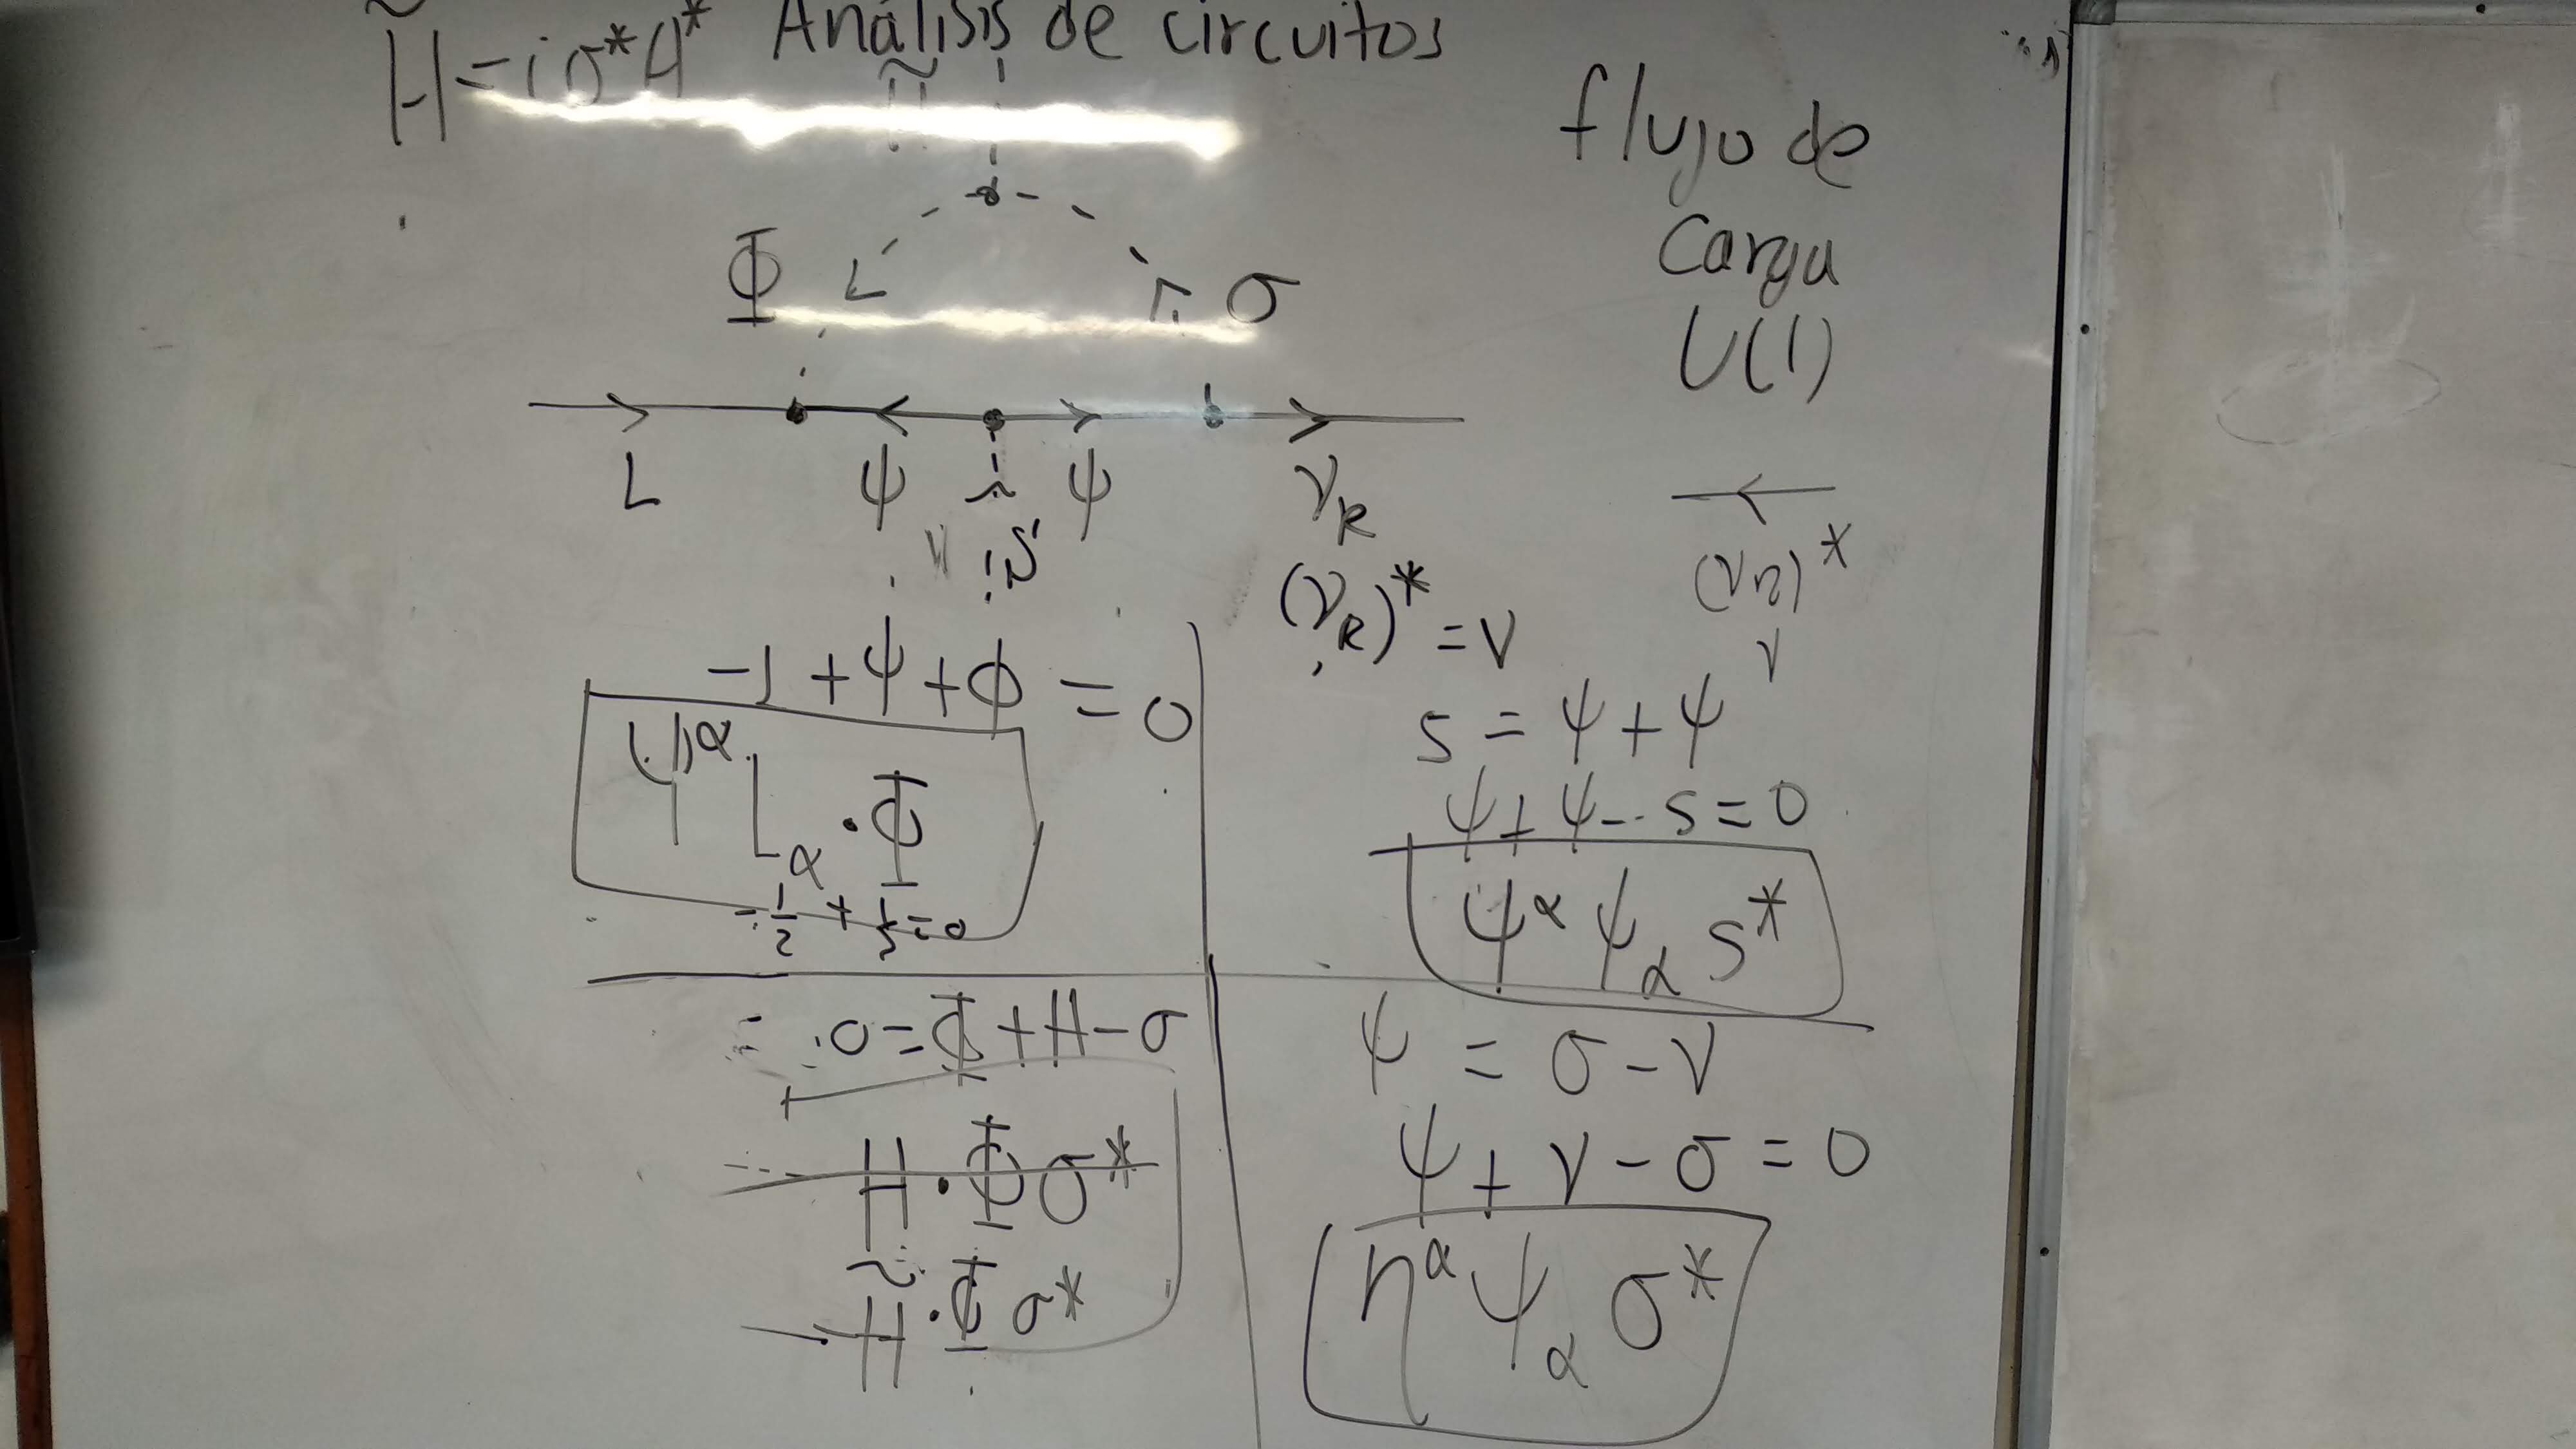
\includegraphics[scale=0.1]{circuito}


\section{Productos escalares}

\section{Diagramas de flujos de cargas}



%%% Local Variables: 
%%% mode: latex
%%% TeX-master: "fullnotes"
%%% ispell-local-dictionary: "castellano8"
%%% End: